\documentclass[acmsmall,screen,review,anonymous]{acmart}

% ============================================================
% Packages (see packages.sty)
% ============================================================
\usepackage{packages}
\microtypesetup{expansion=false}

% ============================================================
% Custom commands (see commands.sty)
% ============================================================
\usepackage{commands}
% =====================================================================
%  SemWeaver shared figure style  (\input after \usepackage{packages})
%  ---------------------------------------------------------------------
%  ONE place that defines the colour palette, node styles and edge
%  styles for every TikZ figure in the paper.  Goals:
%    * colour-blind safe  (blue / orange / teal, never red+green alone)
%    * legible in grayscale print  (hue + line-style redundancy)
%    * font matched to the body text (\footnotesize, no \resizebox)
%  Requires (already in packages.sty): tikz + arrows.meta, positioning,
%  calc, shapes.geometric, fit, backgrounds.
% =====================================================================
\makeatletter
\@ifundefined{swfigurestyleloaded}{\gdef\swfigurestyleloaded{1}}{\endinput}
\makeatother

% ----- Palette --------------------------------------------------------
% Colours sampled from the hand-drawn teaser (fig-overview) and architecture
% (fig-architecture) figures so every TikZ figure shares one visual key:
% soft pastel panels, one bright primary, magenta sub-titles, amber connectors.
\definecolor{swink}{HTML}{1F2329}     % near-black: text / strong strokes
\definecolor{swmuted}{HTML}{5F6874}   % secondary text
\definecolor{swgray}{HTML}{7A828D}    % neutral strokes
\definecolor{swrule}{HTML}{CFD6DF}    % light rules / panel borders
\definecolor{swgrid}{HTML}{ECEFF3}    % very light separators
\definecolor{swmist}{HTML}{F5F7FA}    % neutral fill (inputs / passive)
\definecolor{swwhite}{HTML}{FFFFFF}
% Primary  (process / the tool / main flow) -- PPT dark teal-blue + sky panel
\definecolor{swblue}{HTML}{0B76A0}
\definecolor{swbluefill}{HTML}{E2F5FF}
\definecolor{swbluemid}{HTML}{8BD3F0} % mid blue (box fill / bar fill)
% Accent  (the contribution / "after" / the patch barrier) -- peach
\definecolor{sworange}{HTML}{C0651D}
\definecolor{sworangefill}{HTML}{FBE3D6}
% Safe  (fixed side / silent / accepted) -- PPT green
\definecolor{swteal}{HTML}{1F8A5B}
\definecolor{swtealfill}{HTML}{E6F4DD}
% Danger  (use SPARINGLY; never the sole carrier of meaning)
\definecolor{swred}{HTML}{C23B36}
\definecolor{swredfill}{HTML}{FBE6E3}
% Extra accents harmonised with the redrawn PPT figures
\definecolor{swmagenta}{HTML}{C6154F} % section / sub-title accent (PPT titles)
\definecolor{swamber}{HTML}{FFB300}   % connector arrows / adopt highlight
\definecolor{swlav}{HTML}{ECE8FF}     % lavender fill (bundle / audit)
\definecolor{swpink}{HTML}{FFEBEE}    % gains panel pink
\definecolor{swbadgefill}{HTML}{FFBDC6} % delta-badge fill

% ----- Geometry defaults ---------------------------------------------
\tikzset{
  sw/.style={
    font=\footnotesize,
    >={Latex[length=1.7mm,width=1.5mm]},
    line cap=round, line join=round,
    node distance=6mm and 9mm,
    text=swink,
  },
}

% ----- Node styles ----------------------------------------------------
% base box every node inherits
\tikzset{
  swbox/.style={
    draw=swgray, line width=0.55pt, rounded corners=1.2pt,
    align=center, inner sep=3.2pt, minimum height=7.0mm, font=\footnotesize,
    text=swink,
  },
  swpanel/.style={
    draw=swrule, line width=0.5pt, rounded corners=1.6pt,
    fill=swwhite, inner sep=4.4pt,
  },
  swpaneltitle/.style={font=\scriptsize\bfseries, text=swmuted, anchor=west},
  % passive inputs / artifacts (neutral)
  swio/.style   ={swbox, draw=swgray,    fill=swmist},
  % process steps performed by the tool (primary blue)
  swproc/.style ={swbox, draw=swblue,    fill=swbluefill,   text=swink},
  % the emphasised data object (evidence bundle): heavier blue
  swhub/.style  ={swbox, draw=swblue, line width=0.85pt, fill=swbluefill},
  % contribution / accepted / "after" (accent orange)
  swhi/.style   ={swbox, draw=sworange,  fill=sworangefill},
  % safe / fixed-silent (teal)
  swsafe/.style ={swbox, draw=swteal,    fill=swtealfill},
  % buggy / vulnerable (danger, used sparingly + always with line style)
  swbug/.style  ={swbox, draw=swred,     fill=swredfill},
  % tiny annotation text
  swnote/.style ={font=\scriptsize\itshape, text=swmuted, align=center},
  swcallout/.style={font=\scriptsize, text=swink, align=left},
  swtag/.style  ={font=\scriptsize\bfseries, text=swink},
  swbadge/.style={
    draw=swrule, fill=swmist, rounded corners=5pt,
    inner xsep=3.2pt, inner ysep=1.2pt, font=\scriptsize\bfseries,
    text=swmuted,
  },
  swok/.style   ={font=\footnotesize\bfseries, text=swteal},
  swno/.style   ={font=\footnotesize\bfseries, text=swred},
  swverdict/.style={font=\scriptsize\bfseries\itshape},
  % shared accents matching the redrawn PPT figures
  swptitle/.style={font=\scriptsize\bfseries, text=swmagenta}, % figure sub-titles
  swlavbox/.style={swbox, draw=swblue!55, fill=swlav},         % bundle / audit object
  swmidbox/.style={swbox, draw=swblue, fill=swbluemid},        % emphasised blue box
}

% ----- Code listing style: compact patch diff ------------------------
% Whole-line coloring for removed (vulnerable) and added (fixed) lines,
% redundant with the leading -/+ glyph so it survives grayscale print.
\lstdefinestyle{swdiff}{
  basicstyle=\ttfamily\scriptsize,
  breaklines=false,
  columns=fullflexible,
  keepspaces=true,
  showstringspaces=false,
  numbers=none,
  xleftmargin=4pt, xrightmargin=2pt,
  aboveskip=2pt, belowskip=1pt,
  commentstyle=\color{swmuted}\itshape,
  morecomment=[l]{//},
  moredelim=[il][\color{swred}]{-\ },
  moredelim=[il][\color{swteal}]{+\ },
}

% ----- Edge styles  (hue + dash redundancy for grayscale) -------------
\tikzset{
  swflow/.style    ={-{Latex[length=1.7mm,width=1.5mm]}, draw=swblue,   line width=0.8pt},
  swthin/.style    ={-{Latex[length=1.5mm,width=1.3mm]}, draw=swgray,   line width=0.6pt},
  swaccent/.style  ={-{Latex[length=1.7mm,width=1.5mm]}, draw=sworange, line width=0.9pt},
  swsafeedge/.style={-{Latex[length=1.7mm,width=1.5mm]}, draw=swteal,   line width=0.9pt, dash pattern=on 3pt off 2pt},
  swbugedge/.style ={-{Latex[length=1.7mm,width=1.5mm]}, draw=swred,    line width=0.9pt},
  swfeedback/.style={-{Latex[length=1.5mm,width=1.3mm]}, draw=swgray,   line width=0.6pt, dash pattern=on 2pt off 2pt},
  swamberedge/.style={-{Latex[length=1.9mm,width=1.7mm]}, draw=swamber, line width=1.1pt}, % main connector (PPT amber)
  swrule/.style    ={draw=swrule, line width=0.45pt},
  swrow/.style     ={draw=swgrid, line width=0.35pt},
}

\citestyle{acmnumeric}
\acmConference[FSE 2027]{The ACM International Conference on the Foundations of Software Engineering}{July 12--16, 2027}{Shenzhen, China}
\acmYear{2027}

% ============================================================
% Document
% ============================================================
\begin{document}

\title{\toolname: Refining LLM-Generated Static Vulnerability Checkers with Analyzer-Internal Evidence}

\author{Anonymous Author(s)}

\begin{abstract}
LLM-generated static vulnerability checkers often warn on both vulnerable and fixed code because a patch alone underspecifies guards, state, and data flow.  We study post-synthesis refinement using analyzer-internal representations: backend-produced records bound to raw output and the source revision, file, and function, distinct from diagnostics and source-window fallbacks.  \toolname organizes these records with patch, source, and validation context, accepting an edit only if it retains a vulnerable-side hit while silencing the fixed side.
Among 39 materialized KNighter-derived CSA checkers, 12 are fixed-noisy; their initial 0/12 patch-discriminating success (PDS) is a selection criterion, not KNighter's refinement performance.  Across three full-feedback repeats with matched per-case call ceilings on these 12 Linux cases, KNighter's actual loop achieves 3, 2, and 6 PDS; native-evidence \toolname achieves 6, 5, and 7, while its no-internal arm achieves 3 each time.  Under PDS-only adoption, native \toolname retains 23, 23, and 18 of 37 starting fixed-side alerts versus KNighter's 28, 27, and 22.  Of 70 evidence records, 37 meet the strict internal definition.  These development-informed repeated results indicate bounded patch-local false-positive reduction; no individual paired difference is significant, and no unseen-code generalization is claimed.

\end{abstract}
\maketitle

% ============================================================
% Main body (FSE 2027: up to 18 pages of text and figures)
% ============================================================

\section{Introduction}\label{sec:intro}
Static analysis is a cornerstone of software security assurance for systems code.
Tools such as CodeQL~\cite{codeqlDocs} and Clang Static Analyzer (CSA)~\cite{clangsaDocs} detect vulnerabilities by checking source code against predefined rules without executing it~\cite{engler2001bugs,bessey2010coverity,calcagno2015infer,sadowski2015tricorder}.
The effectiveness of these tools depends on the quality of their vulnerability checkers, each of which must encode the semantic conditions (path guards, state invariants, data-flow relations, and API contracts) that distinguish a real bug from safe code.
Writing such checkers by hand requires deep expertise in both the target codebase and the analysis framework, making manual authoring expensive, slow, and difficult to scale.

LLM-based patch-driven synthesis offers a promising alternative.
In this paradigm, a security patch serves as a compact before/after specification: the LLM consumes the patch and synthesizes a reusable checker that should fire on the vulnerable revision but remain silent on the fixed revision.
KNighter~\cite{yang2025knighter}, a representative system, has demonstrated that this approach can produce compilable and executable CSA checkers from historical Linux kernel fixes.

However, the resulting checkers may be semantically inadequate.
A security patch is inherently underspecified: a one-line \texttt{goto}-target change may encode an ownership barrier, a widened cast may encode a range guard, and a moved \texttt{free} may encode a lifetime invariant.
A checker that captures only the syntactic shape of the edit, without encoding the underlying semantic condition, can fire on both the vulnerable and fixed revisions.
After na\"ive refinement, the checker may instead lose the vulnerable-side trigger entirely, a failure mode we call over-pruning.
In both cases the root cause is the same: the checker learned the syntactic edit but not the semantic condition it enforces.

Current refinement strategies, including KNighter's own iterative loop, attempt to address this problem by operating at the output level~\cite{yang2025knighter,madaan2023selfrefine,shinn2023reflexion}.
They run the checker on both revisions, observe whether it fires on the wrong side, and feed this behavioral signal back to the LLM.
Such feedback reveals the symptom (``the fixed side still warns'') but does not diagnose the cause: it cannot tell the LLM whether the missing predicate is a path guard, a cleanup barrier, an ownership transition, or an API contract.
The LLM must therefore guess the missing semantic condition, reducing refinement to prompt-level retry.

We make a narrower observation: \textbf{some patch-relevant program structure is available in analyzer-produced intermediate representations} but is not ordinarily surfaced to the refinement loop.
Path-sensitive analyzers such as CSA internally track branch guards, symbolic states, memory regions, and lifetime events during checker execution~\cite{clangsaDocs}.
Relational query engines such as CodeQL maintain databases of data-flow edges, call-graph relations, type hierarchies, and API-usage patterns~\cite{avgustinov2016ql,codeqlDocs}.
These representations can suggest candidate predicates, but a CFG edge or call relation is not by itself a proof of path feasibility or checker correctness.

Exploiting these intermediate results, however, is not straightforward.
A single CSA run can produce hundreds of path-sensitive states, and a CodeQL database exposes thousands of relational tuples.
Feeding all of them into the refinement prompt overwhelms the context window, dilutes the relevant facts with noise, and makes it harder for the model to identify the specific predicate that needs to be added.
The challenge is to select and present only the evidence that is relevant to the particular semantic gap in the checker under refinement.

We present \toolname, a post-synthesis checker editor guided by provenance-labelled analyzer context.
\toolname is designed as a plug-in post-generation layer that is independent of the upstream LLM generator, treating any generated checker (from KNighter or another pipeline) as an artifact to be refined rather than regenerated.
The framework addresses the evidence-selection challenge through three mechanisms.
First, a rule-guided preflight extracts patch facts (e.g., guards, type widening, and affected calls) and prioritizes evidence requirements by inferred mechanism.  The editor may request role views in the general workflow; the strict CSA comparison instead freezes its patch-scoped view before editing.
For instance, a cleanup-edge patch triggers collection of path-guard and lifetime evidence from CSA, while a bounds patch triggers guard, flow, and API-usage evidence from CodeQL.
Second, backend outputs, patch facts, source context, and validation feedback are normalized into a compact bundle with typed records, giving the editor a structured edit target (``add the patch-introduced cleanup barrier while preserving the freed-object transition'') instead of a vague behavioral symptom (``fixed side still warns'').
Third, a strict target-preserving gate accepts a refinement only when the refined checker both preserves the vulnerable-side trigger and eliminates the fixed-side warnings, preventing over-pruning by construction.

We evaluate \toolname across three settings.
We screen all 39 materialized KNighter-derived Linux CSA checkers: 12 are fixed-noisy and form the refinement stratum, while already-discriminating checkers remain in the portfolio denominator.  The selected stratum's initial 0/12 is definitional, not a KNighter refinement baseline.  A historical follow-up has five automatic PDS edits, six manual completions, and one loss, but predates strict analyzer-internal evidence.  In three later, matched full-feedback repeats, the actual KNighter loop reaches 3, 2, and 6 PDS on the 12 cases; provenance-gated \toolname reaches 6, 5, and 7, retaining fewer fixed-side alerts in each repeat under PDS-only adoption.  The no-internal arm reaches 3 each time.  These are descriptive results on the same selected cases, not significant per-repeat superiority or unseen-code generalization; historical cross-backend and one-run model results remain exploratory.

This paper makes the following contributions:
\begin{itemize}
  \item We identify the gap between output-level behavioral feedback and analyzer-internal semantic evidence for checker refinement, and formulate the problem of target-preserving semantic refinement for LLM-generated vulnerability checkers.
  \item We present \toolname, a plug-in refinement layer that organizes provenance-labelled analyzer representations, analyzer outputs, patch and source context, and validation feedback into a compact semantic evidence bundle; the strict CSA comparison freezes the available view rather than evaluating adaptive routing.
  % \item We design a strict target-preserving validation gate that prevents over-pruning, and demonstrate its necessity through ablation.
  \item We provide a denominator-complete audit of KNighter-derived Linux checkers and separate historical, matched-budget, cross-backend, ablation, and failure-analysis results by their provenance and inferential scope.
\end{itemize}


\section{Background}\label{sec:background}
This section introduces the background on static vulnerability checkers, LLM-based checker generation from security patches, and the analyzer-internal intermediate results that motivate our approach.

\subsection{Static Vulnerability Checkers}

Static analysis examines source code without executing it, aiming to find bugs, security vulnerabilities, and code-quality issues at compile time or during code review~\cite{engler2001bugs,bessey2010coverity}.
A vulnerability checker is a rule or query within a static-analysis framework that flags program locations matching a security-relevant condition.
Modern frameworks support different checker paradigms.
Path-sensitive engines such as the Clang Static Analyzer (CSA) perform symbolic exploration over program paths, tracking branch guards, symbolic values, memory regions, and lifetime transitions to detect bugs like use-after-free, null dereference, and resource leaks~\cite{clangsaDocs}.
Relational query engines such as CodeQL compile source code into a queryable database and express checkers as declarative queries over data-flow edges, call-graph relations, type hierarchies, and API-usage patterns~\cite{avgustinov2016ql,codeqlDocs}.
Both paradigms have been deployed at industrial scale for continuous vulnerability detection~\cite{sadowski2015tricorder,calcagno2015infer}.

Writing effective checkers remains a bottleneck.
A checker must encode not only the syntactic pattern of a vulnerability but also the semantic conditions (path guards, state invariants, data-flow relations, and API contracts) that distinguish real bugs from safe code.
This requires deep domain knowledge of both the target codebase and the analysis framework, making manual checker authoring expensive and error-prone.

\subsection{LLM-Based Patch-Driven Checker Generation}

Recent work has proposed using LLMs to automate checker generation from security patches.
A security patch provides a compact before/after specification: the vulnerable revision should trigger the generated checker, and the fixed revision should not.
This idea builds on a well-established line of work that treats patches as vulnerability specifications, including semantic patching~\cite{padioleau2008coccinelle}, clone-based vulnerability discovery~\cite{jang2012redebug,kim2017vuddy}, and patch-derived datasets~\cite{fan2020bigvul}.
KNighter~\cite{yang2025knighter} is a representative system that synthesizes CSA checkers from historical Linux kernel fixes and validates them against the vulnerable and fixed revisions.

However, the generated checkers are seldom semantically adequate.
A patch is inherently underspecified: a one-line edit may encode a path guard, an ownership transition, a lifetime barrier, or an API contract, yet the generated checker often captures only the syntactic shape of the edit without the semantic condition the edit enforces.
Existing refinement loops, including KNighter's own iterative strategy, operate at the output level~\cite{yang2025knighter,madaan2023selfrefine,shinn2023reflexion}.
They feed behavioral signals (e.g., ``the fixed side still warns'') back to the LLM, revealing the symptom but not diagnosing the cause.
This feedback cannot tell the LLM whether the missing predicate is a path guard, a cleanup barrier, an ownership transition, or an API contract, so the model must guess which semantic condition to add.

\subsection{Analyzer-Internal Intermediate Results}

Static-analysis backends compute intermediate representations that can be exposed through debugging interfaces or database queries, but these are not normally supplied to a checker-refinement loop.

CSA, as a path-sensitive engine, internally maintains per-path symbolic states that record branch conditions, memory region bindings, allocation/free events, and object lifetime transitions~\cite{clangsaDocs}.
CodeQL, as a relational engine, materializes a full program database from which data-flow edges, call-graph relations, type hierarchies, member-access patterns, and API-usage sequences can be queried~\cite{avgustinov2016ql,codeqlDocs}.
These intermediate facts have long underpinned taint analysis, graph-based detection, and interprocedural security reasoning~\cite{livshits2005finding,jovanovic2006pixy,arzt2014flowdroid,yamaguchi2014cpg}.

These representations may suggest a missing predicate, but a CFG branch or database tuple does not itself establish vulnerability semantics.
The operational distinction between a backend-produced representation, a diagnostic, and a source-window fallback is central to our evidence accounting (Section~\ref{sec:evidence-roles}).
This motivates extracting bounded, provenance-labelled context for refinement while retaining paired validation as the correctness gate.


\section{Motivating Example}\label{sec:motivating}
Consider the KNighter-derived CSA checker for Linux commit
\texttt{5aa2184e2908}, which fixes a double-free error path in
\lstinline|mlx5hws_definer_calc_layout|~\cite{linuxCommit5aa2184e,yang2025knighter}.
Figure~\ref{fig:motivating} shows two fallible calls: conversion helper
\lstinline|hws_definer_conv_match_params_to_hl| (\cmark{1}) establishes
ownership of \lstinline|mt->fc| only on success; a later layout-fitting
failure may then legitimately release it through \lstinline|free_fc|.
On conversion failure, however, the vulnerable \lstinline|goto| targets
\lstinline|free_fc| (\cmark{2}) before ownership exists.  The patch
redirects only that edge to \lstinline|free_match_hl| (\cmark{4}),
which frees the already-owned \lstinline|match_hl| while bypassing
\lstinline|mt->fc|.  The needed predicate distinguishes these guarded
error paths, not merely the presence of a free call.

% Current figure design:
%   Panel A: patch hunk with M1--M21 labels.  Solid arrows are real patch
%   control flow; dashed arrows are checker-to-code mappings.  Orange marks the
%   unsafe/report path, teal marks the refined/barrier path, and gray marks
%   generic scanning or legitimate later control flow.
%   Panel B: baseline broad allocation/free checker with B1--B14 labels and
%   strict-validation outcome 10/9.
%   Panel C: refined path/state predicate with C1--C15 labels and
%   strict-validation outcome 1/0.
\begin{figure*}[t]
  \centering
  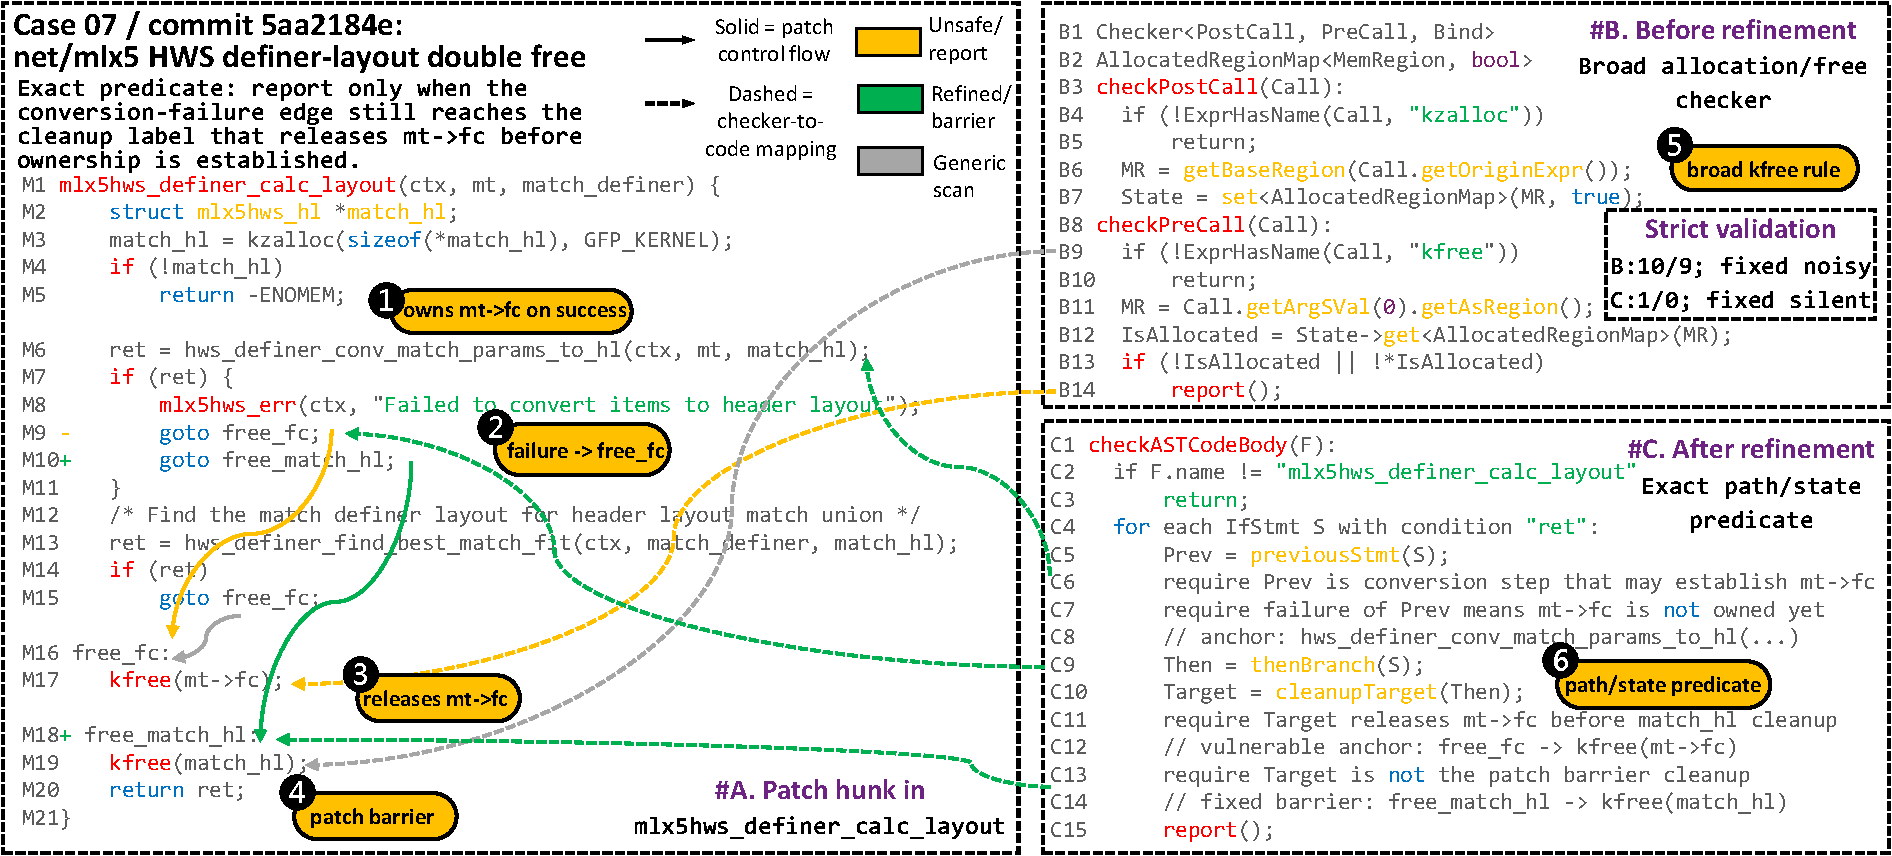
\includegraphics[width=\textwidth]{figures/fig-motivating.pdf}
  \Description{Three-panel example showing the vulnerable and fixed cleanup edges, the broad starting checker with ten and nine alerts, and a manually completed patch-bound checker with one and zero alerts.}
  \caption{\textbf{Motivating double-free refinement.}
  Solid arrows show patch control flow. Dashed arrows show
  checker-to-code mappings.  Orange highlights the unsafe path,
  teal the patched barrier, and gray the legitimate later flow.
  The baseline checker (\cmark{5}) fires broadly (\texttt{10/9}).
  The manually completed checker (\cmark{6}) encodes the conversion-failure
  ownership predicate and achieves \texttt{1/0}; this case is not an
  automatic-refinement success.}
  \label{fig:motivating}
\end{figure*}

\textbf{Checker behavior and evidence.}
The starting checker (\cmark{5}) tracks \lstinline|kzalloc| regions
and warns at \lstinline|kfree| when a region is absent from its map.
It misses the guarded ownership distinction and emits \texttt{10/9}
patch-local alerts on vulnerable/fixed revisions.  A fixed-side report
shows the symptom but does not identify the conversion call, guard,
cleanup edge, and owned object that form the separator.  The evidence
bundle places the two cleanup labels and guarded edges in one semantic
slice; a Clang CFG dump supports branch context, while the ownership
interpretation comes from patch and source analysis, \emph{not} a
path-feasible analyzer proof.  A validation-only edit can simply suppress
both sides: the historical one-run ablation here produced \texttt{0/0}.

The checker in Figure~\ref{fig:motivating}c was \emph{manually completed}:
its AST-body predicate recognizes the conversion-failure edge and changes
paired counts to \texttt{1/0}.  It is not an automatic \toolname success.
Modeling the allocator or tracked-state check in the original symbolic
checker would be another plausible repair; this example does not show
that the AST rewrite is preferable.  The shown predicate names the patch
function and is therefore patch-bound, not a general double-free detector.
The strict PDS gate establishes only the paired result, not stability
under future changes to the code or callback names.


\section{Approach}\label{sec:approach}
\toolname is a post-synthesis refinement layer for LLM-generated vulnerability detectors.  Given a draft CSA checker or CodeQL query produced by an upstream generator, the patch that motivated the synthesis, and the corresponding source tree and validation scope, \toolname refines the detector to encode missing semantic predicates while preserving the vulnerable-side trigger.

% \subsection{Overview}

\begin{figure*}[t]
  \centering
  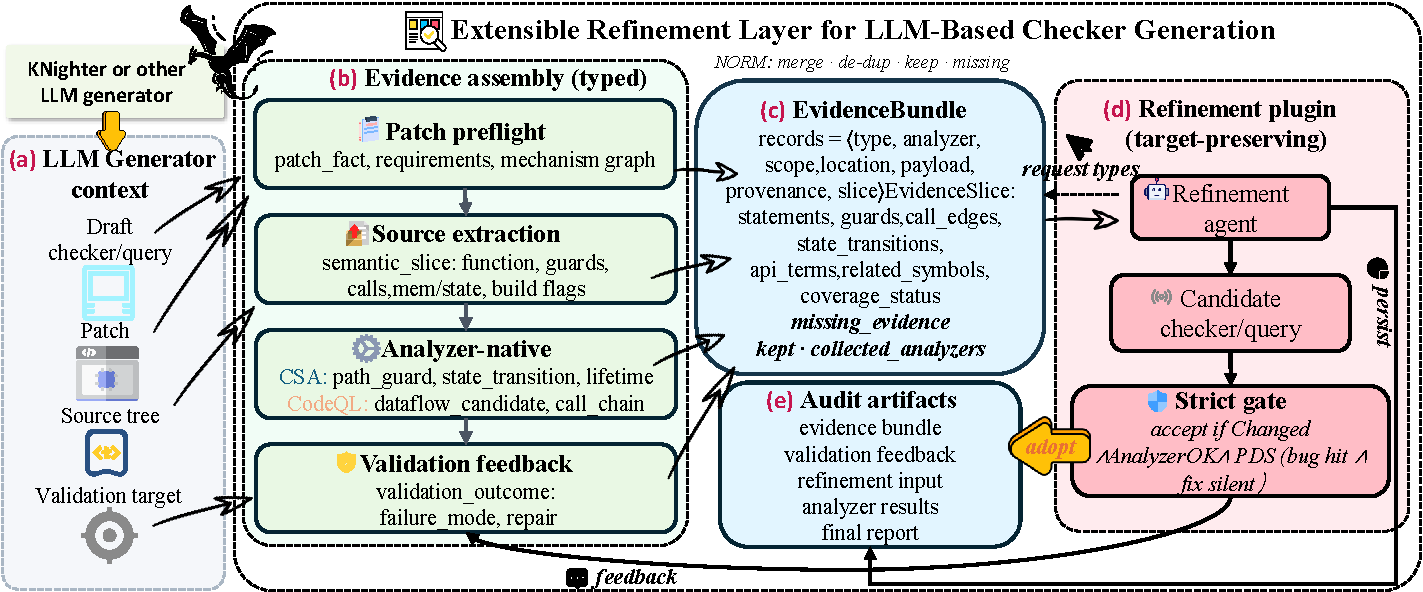
\includegraphics[width=\textwidth]{figures/fig-architecture.pdf}
  \Description{Workflow from a generated checker and patch through evidence collection, a typed provenance-labelled bundle, checker editing, paired validation, and audit artifacts.}
  \caption{\textbf{\toolname architecture.}
  (a)~An LLM generator produces a draft detector from the patch.
  (b)~A rule-guided patch preflight plans evidence requirements and four collectors gather corresponding facts; the figure's ``analyzer-native'' collector label does not mean every emitted record has internal provenance.
  (c)~Facts are normalized into a typed \texttt{EvidenceBundle} with seven persisted record types.
  (d)~The refinement agent edits the detector using role-specific views. A strict gate accepts only candidates that preserve the vulnerable-side trigger while silencing the fixed side. Rejected candidates feed back into the bundle (dashed arrow).
  (e)~Adopted candidates, evidence bundles, and validation logs are persisted as audit artifacts for reproducibility.}
  \label{fig:approach-architecture}
\end{figure*}

Figure~\ref{fig:approach-architecture} shows five stages.
\textbf{(a)~Generator context.}  \toolname receives a draft detector from an upstream LLM generator (e.g., KNighter), together with the patch, source tree, and validation target.  It treats the generator as a black box: any synthesized detector is an artifact to be refined, not regenerated.
\textbf{(b)~Evidence assembly.}  Rule-guided patch preflight infers a likely mechanism from patch facts and available analysis metadata, then prioritizes evidence requirements.  Four collectors (patch preflight, source extraction, analyzer representations or outputs from CSA/CodeQL, and validation feedback) gather evidence (Section~\ref{sec:adaptive-selection}).
\textbf{(c)~Evidence bundle.}  All facts are normalized into a typed \texttt{EvidenceBundle} with seven persisted record types, giving the refinement agent structured edit targets rather than raw analyzer dumps (Sections~\ref{sec:evidence-roles} and~\ref{sec:evidence-schema}).
\textbf{(d)~Target-preserving refinement.}  The refinement agent edits the detector using role-specific evidence views from the bundle.  A strict gate accepts a candidate only when it preserves the vulnerable-side trigger and eliminates fixed-side warnings.  Rejected candidates re-enter the bundle as feedback for the next iteration (Section~\ref{sec:refinement}).
\textbf{(e)~Audit artifacts.}  Each run persists the starting and candidate detector, evidence bundle, prompt/response trace, validation logs, and final report.  The verifier recomputes raw-output hashes, checks the recorded Clang interface/schema and patch file/function binding for every internal record, recounts provenance classes, and then checks the compiled candidate against paired vulnerable/fixed logs.  It does not infer evidence origin from an LLM explanation or rerun a model to reproduce a deterministic count.

\begin{algorithm}[t]
\footnotesize
\caption{Target-Preserving Evidence-Guided Refinement}
\label{alg:evidence-guided-refinement}
\begin{algorithmic}[1]
\Require detector $D$, patch $P$, source $S$, scope $V$, backends $A$, budget $K$
\Ensure refined detector $D^*$ and audit report
\State $R_0 \gets \Call{Validate}{D,P,V}$
\State $E_p,E_s \gets \Call{Preflight}{P},\ \Call{ExtractSource}{P,S,D}$
\State $E_a \gets \bigcup_{a\in A}\Call{CollectNative}{a,D,P,S}$ \quad $E_v \gets \Call{Feedback}{R_0}$
\State $B \gets \Call{NormalizeMerge}{E_p,E_s,E_a,E_v}$
\If{$\Call{PDS}{D,P,V}$}
  \State \Return $\Call{Audit}{D,B}$
\EndIf
\State $D^* \gets D$
\For{$i=1$ to $K$}
  \State $V_i \gets \Call{AgentSelectView}{B}$ \quad $C_i \gets \Call{AgentEdit}{D^*,P,V_i}$
  \State $R_i \gets \Call{Validate}{C_i,P,V}$
  \If{$\Call{Changed}{C_i,D^*} \land \Call{AnalyzerOK}{R_i} \land \Call{PDS}{C_i,P,V}$}
    \State $D^* \gets C_i$ \quad \textbf{break}
  \Else
    \State $E_i \gets \Call{Feedback}{R_i}$ \quad $B \gets \Call{Merge}{B,E_i}$
  \EndIf
\EndFor
\State \Return $\Call{Audit}{D^*,B}$
\end{algorithmic}
\end{algorithm}

\subsection{Adaptive Evidence Selection}
\label{sec:adaptive-selection}

The central design choice in evidence assembly~(Figure~\ref{fig:approach-architecture}b) is \emph{what to collect and expose}.  Analyzer outputs can be large and heterogeneous; passing them wholesale to the editor obscures patch-relevant relations.  The preflight planner represents candidate requirements by role and priority, while source/function scope and bounded views limit what the editor sees.  In the strict CSA comparison, collection is precomputed and the visible view is frozen, so its result does not measure demand-driven routing.

\textbf{Rule-guided preflight and role requests.}
The implementation has no separately trained or prompted patch-mechanism classifier.  \texttt{PatchFacts\allowbreak Extractor} parses the patch and metadata for affected functions, added guards, risky calls, and type widenings.  \texttt{Evidence\allowbreak Planner} takes a primary pattern from analysis metadata when available or infers it from those facts, then assigns fixed priorities to requirements: patch anchoring is 100, lifetime/state requirements for double-free or use-after-free are 92/89, and a guard for null or bounds cases is 90.  It sorts by descending priority with evidence type as a tie-breaker and retains at most eight planned requirements in the default configuration.  Table~\ref{tab:evidence-routing} summarizes mechanism-to-role examples; it is not a classifier confusion matrix or a promise that every role is analyzer-internal.  The normalizer does not learn or re-rank facts.  In the general workflow the editor may request evidence types, with duplicate and request-count limits.
For the strict provenance-audited CSA comparison, patch-scoped records are precomputed.  The treatment preloads up to the first four distinct strictly internal record types in persisted order and disables additional requests; its no-internal counterpart sees no internal records but retains patch, source, and feedback context.  This deterministic exposure policy is a limitation, not an adaptive classifier.  The matched result tests the frozen native-evidence view, \emph{not} a routing policy's accuracy or benefit.

\begin{table}[t]
\footnotesize
\centering
\setlength{\tabcolsep}{3pt}
\caption{Rule-guided evidence requirements by patch mechanism (representative); names are persisted record types, not gold labels or measured classifier outputs.}
\label{tab:evidence-routing}
\begin{tabular}{@{}p{0.32\columnwidth}p{0.40\columnwidth}p{0.18\columnwidth}@{}}
\toprule
\textbf{Patch mechanism} & \textbf{Possible record types} & \textbf{Backend} \\
\midrule
Cleanup edge / double free & \texttt{allocation\_lifecycle}, \texttt{state\_transition}, \texttt{path\_guard} & CSA \\
Bounds widening / overflow & \texttt{semantic\_slice}, \texttt{dataflow\_candidate}, \texttt{state\_transition} & CSA/CodeQL \\
Initialization / null deref & \texttt{state\_transition}, \texttt{path\_guard} & CSA \\
Use-after-free / escape & \texttt{allocation\_lifecycle}, \texttt{call\_chain} & CSA/CodeQL \\
API misuse / missing check & \texttt{semantic\_slice}, \texttt{call\_chain} & CodeQL \\
\bottomrule
\end{tabular}
\end{table}

\subsection{Evidence Sources and Roles}
\label{sec:evidence-roles}

Given the patch scope and any planned requirements, four collectors execute in sequence (Figure~\ref{fig:approach-architecture}b, top to bottom):

\textbf{Patch preflight} identifies changed files, hunks, and statements, and produces a mechanism graph that links the edited code to likely bug patterns.  This supplies the structural skeleton: \emph{what changed} and \emph{where}.

\textbf{Source extraction} resolves patch files and records bounded contexts around the changed code, including enclosing functions, branch guards, callee signatures, memory/state operations, and build flags.  This provides local semantic context without dumping repository-scale source.

\textbf{Analyzer evidence} is classified by its actual origin, not by the collector's name.  We call a record \emph{analyzer-internal} only if its payload is derived from a backend-produced intermediate representation, identifies the interface and raw output, and is bound to a source revision, file, and function.  In the measured CSA cohort the interface is Clang 18's \texttt{debug.DumpCFG} and \texttt{debug.DumpCallGraph}; the persisted UTF-8 dump is parsed into schema \texttt{semweaver.csa\_cfg\_snapshot.v1}, with a raw-output SHA-256 and source-scope binding.  These dumps provide CFG branches and value bindings and call edges.  They do \emph{not} themselves prove a path-feasible lifetime or ownership transition.  Analyzer diagnostics and alert counts are \emph{analyzer output}, not internal state.  Patch diffs, source windows, and compile-database-assisted source extraction are \emph{source-derived} fallbacks even when a CSA or CodeQL collector emits them.  A live CodeQL database query could meet the internal-evidence definition if its query, database revision, and tuples were retained; we do not attribute source-window-derived CodeQL facts to that category.

This distinction makes extraction challenging in a practical sense: backend intermediates are verbose, backend-specific, sometimes unavailable for the patch-related translation unit, and must be linked to the same revision and function as the checker failure.  The collector retains missing-evidence markers rather than silently upgrading fallback source text to internal evidence.  Across the 12 CSA evidence bundles used in the provenance audit, 55 of 70 records are analyzer-produced: 37 meet the strict internal definition and 18 are analyzer outputs; the remaining 15 are source-derived.  All 37 internal records have raw-dump and patch-scope bindings in the audit.  These counts characterize evidence availability, not refinement success or CodeQL-native coverage.

\begin{table}[t]
\centering\footnotesize
\setlength{\tabcolsep}{3pt}
\caption{Evidence primitives and provenance in the audited 12-case CSA cohort.  One record may contain several CFG primitives; counts are by record origin, not primitive.}
\label{tab:origin-types}
\begin{tabular}{@{}p{0.27\columnwidth}p{0.53\columnwidth}r@{}}
\toprule
Origin & What the persisted record contains & Records \\
\midrule
Analyzer-internal & Clang CFG branches/guards, value bindings, and call-graph edges, bound to raw dump and function & 37 \\
Analyzer output & CSA diagnostics and paired validation reports; no internal state & 18 \\
Source-derived & Patch facts, source windows, or compile-database-assisted slices & 15 \\
\bottomrule
\end{tabular}
\end{table}

\textbf{Validation feedback} records whether the baseline detector compiles, executes, hits the vulnerable target, remains fixed-side noisy, or loses the target entirely.  This provides the failure \emph{symptom}, while the preceding three sources supply the semantic \emph{edit target}.

% \smallskip
The persisted type vocabulary is \texttt{patch\_fact}, \texttt{semantic\_slice}, \texttt{dataflow\_candidate}, \texttt{call\_chain}, \texttt{path\_guard}, \texttt{allocation\_lifecycle}, and \texttt{state\_transition}.  A \texttt{patch\_fact} anchors changed statements; \texttt{semantic\_slice} summarizes bounded statements, guards, API terms, and related symbols.  \texttt{dataflow\_candidate} and \texttt{call\_chain} describe possible propagation and call context, while \texttt{path\_guard}, \texttt{allocation\_lifecycle}, and \texttt{state\_transition} describe control, resource, and abstract-state context.  ``Barrier,'' ``type filter,'' and ``API usage'' are semantic interpretations inside these records, not additional persisted types or claims of proven path feasibility.

When a selected role yields no evidence, the bundle retains an explicit missing-evidence marker rather than treating the absence silently, so the refinement agent knows what was requested but unavailable.

\subsection{Evidence Bundle Schema}
\label{sec:evidence-schema}

The normalizer merges all collected facts into the \texttt{EvidenceBundle} shown in Figure~\ref{fig:approach-architecture}c.  Each fact becomes an \texttt{EvidenceRecord} carrying a type, the contributing analyzer, scope, source location, payload, provenance, and an optional \texttt{EvidenceSlice} (the compact semantic content consumed by the agent).  The schema separates program facts from analysis rules in the spirit of relational analyzer frameworks~\cite{avgustinov2016ql,jordan2016souffle,bravenboer2009doop}, but uses a smaller role vocabulary tailored to checker refinement.  Formally:
\begin{equation}
\begin{aligned}
B &= \mathrm{Norm}(E_p \cup E_s \cup E_a \cup E_v),\\
E_a &= E_{\mathrm{CSA}} \cup E_{\mathrm{CodeQL}},\\
r &\in B.records = \langle type, analyzer, scope,\\
&\quad location, payload, provenance, slice\rangle.
\end{aligned}
\label{eq:evidence-bundle}
\end{equation}
Here $E_p$ contains patch facts (changed statements, inferred bug mechanism), $E_s$ contains bounded source slices around the patch and detector trigger, $E_a$ contains analyzer-internal representations \emph{or} analyzer outputs filtered by selected roles (Section~\ref{sec:adaptive-selection}), and $E_v$ contains validation outcomes.  Each record's \texttt{provenance.origin} distinguishes \texttt{analyzer\_internal}, \texttt{analyzer\_output}, and \texttt{source\_derived}.  The normalizer deduplicates records and retains explicit markers for missing evidence; a record's origin is not a confidence score or a proof of semantic correctness.

The type-to-backend mapping reflects available interfaces: CSA CFG/call-graph dumps inform guard, state, and call-chain records; CodeQL queries can support flow and relation records when a live database is available.  These are record types, not seven distinct backend analyses.  Cross-function call edges provide context, but the present CSA dump does not establish an interprocedural path or ownership proof.  Provenance remains visible when a type is populated only by a fallback.

The bundle is bounded by design: preflight requirements and collectors restrict scope to patch-related files and validation targets, while the editor receives selected or preloaded role views rather than the full raw dump (Figure~\ref{fig:approach-architecture}d).  These constraints control prompt size and allow the contribution of strictly internal records to be tested by a matched ablation.  A small, single-run ablation cannot by itself establish their causal contribution across the cohort.

\subsection{Target-Preserving Refinement}
\label{sec:refinement}

The refinement loop (Figure~\ref{fig:approach-architecture}d) receives the current detector, patch, baseline validation notes, and a bounded role-specific evidence view.  The interface supports requesting further roles from the persisted bundle (``request types'' arrow), but the provenance-audited matched condition freezes the visible view before the edit and disables additional agent requests.  Thus its measured effect is a contrast between preselected native-evidence and no-internal views, not a test of dynamic evidence retrieval.  This keeps the prompt bounded and the two conditions auditable.

The agent's tool-mediated loop draws on recent LLM agent and self-refinement architectures but constrains actions to attached evidence, detector edits, and validation commands~\cite{madaan2023selfrefine,shinn2023reflexion,yao2023react,schick2023toolformer}.  Where evidence requests are enabled, they replay attached records rather than launch open-ended repository exploration; the request count is capped and unused or missing evidence is logged.  In the matched condition, request count is zero by protocol.

\textbf{Model versus deterministic components.}  LLMs may produce patch-analysis metadata and the editor's checker edit; when enabled, the editor also chooses which evidence types to request.  The preflight requirement rules, raw-output hashing and scope binding, record normalization, checker compilation, paired replay, and acceptance are programmatic.  The LLM does not create a backend dump, set a provenance origin, or decide PDS.  The audit retains the exact starting checker, prompt and response, visible roles, raw evidence, candidate source, and validation decision.  This boundary prevents an LLM explanation from being counted as analyzer-produced evidence.
The editor prompt supplies the current and starting checker paths, patch path, bounded source/evidence view, baseline vulnerable/fixed symptom, backend identity, and edit/validation rules.  It asks for an in-place checker edit that models the mechanism rather than matching patch spellings, forbids suppressing the vulnerable trigger, and requires compilation before paired acceptance.  Compiler-repair prompts receive the actual build diagnostics; all available English templates and rendered exchanges are named in the artifact manifest, with absent historical raw exchanges explicitly marked rather than reconstructed.

\textbf{Strict gate.}  \toolname treats validation as both an analyzer-facing and a semantic gate (``Strict gate'' in Figure~\ref{fig:approach-architecture}d).  A candidate must satisfy three conditions: (1)~it has changed relative to the previous detector, (2)~it compiles and executes under its backend harness (\textsc{AnalyzerOK}), and (3)~it achieves patch-discriminating success (PDS), i.e., it reports the target on the vulnerable revision while remaining silent on the fixed revision.  If a candidate becomes fixed-side silent by losing the vulnerable-side report, \toolname records a validity loss rather than a success, preventing over-pruning.

\textbf{Feedback loop.}  When the gate rejects a candidate, the validation outcome is fed back into the bundle as new evidence (feedback arrow in Figure~\ref{fig:approach-architecture}), enriching subsequent refinement attempts with the specific failure mode (e.g., ``lost vulnerable-side trigger at line~X'').  The loop terminates when a candidate passes the gate or the budget $K$ is exhausted (Algorithm~\ref{alg:evidence-guided-refinement}).
The repeated call-matched profile used below freezes the evidence view and submits at most one model edit before each external vulnerable/fixed replay.  If the candidate fails the local build or the paired gate, the next permitted call receives hash-bound compiler or paired-alert feedback; the first strict PDS candidate stops the case.  Its per-case ceiling is set by the actual KNighter model calls in the same repeat.  An earlier 19-call diagnostic performed paired replay only after the editor session and cannot measure this iterative-feedback profile; we do not pool its result with the repeats.

The concrete backend depends on the detector type: CSA checkers are compiled and replayed against both revisions, while CodeQL queries run over the pre-built database.  Adding a backend requires an extractor that persists raw output and provenance fields, a mapping to editor-facing roles, and a paired validator that supplies the same $H_v/S_f$ decision.  Adding a bug mechanism requires a routing example, relevant role mapping, and paired positive/negative fixtures; it does not automatically require a new analyzer primitive.  We have not measured engineer-hours for either extension and do not claim zero integration cost.

% \subsection{Outputs}

% Each run writes the refined detector, normalized evidence bundle, preflight plan, validation feedback, refinement manifest, analyzer result records, and final report, so a refinement instance can be audited or resumed without reconstructing experiment state.


\section{Evaluation}\label{sec:evaluation}
We evaluate \toolname's patch-related false-positive reduction and its sensitivity to verified analyzer-internal records.  The scope is paired patch revisions and related build objects, not whole-kernel bug discovery.

\subsection{Research Questions}

\textbf{RQ1: KNighter-derived checkers.} Can \toolname improve strict patch discrimination for external CSA checkers derived from KNighter artifacts?

\textbf{RQ2: Cross-backend feasibility and provenance.} Which detector formats can the layer process, and what can the historical independent-generator data support once manual construction and missing lineage are accounted for?

\textbf{RQ3: Evidence sensitivity.} What changes when strict analyzer-internal records are withheld under an otherwise matched feedback protocol?

\subsection{Subjects}

We distinguish E1 (KNighter-derived Linux CSA checkers), E2 (historical cross-backend feasibility), and E3 (evidence sensitivity).  The old five-case, single-run model study is retained in the artifact but excluded from effectiveness claims.

We start from the frozen, materialized 39-checker KNighter evaluation cohort, not only cases selected for refinement; this is \emph{not} the universe of all checker candidates.  After correcting a failed-analyzer validation for memory-leak commit \texttt{27834971}, 27 checkers already satisfy PDS and 12 have a vulnerable-side hit but remain fixed-noisy.  The 12 are the complete observed fixed-noisy stratum \emph{within this cohort}, not a random or held-out sample.  Their baseline PDS of $0/12$ is definitional; it is \emph{not} KNighter's refinement performance.  We retain the 39-checker denominator for portfolio-level reporting, and separately report the fixed-noisy stratum to measure how often the post-synthesis layer can remove its observed warnings.
The frozen 39 include six local-triage, 17 positive-scan-selected, and 16 valid-but-no-local-report candidates across ten bug families; they are not a random sample.  In a separate inventory of 286 generated artifacts, 45 carried an older \texttt{score\_valid} flag, 35 overlapping the 39.  All ten non-overlapping final-checker files were empty, so we explicitly substituted hash-bound repaired files and replayed the same paired object scope.  Five already meet PDS, two are fixed-noisy, and three miss the vulnerable target; all ten executed.  The resulting 49-commit union is a screening extension, \emph{not} the 12-case matched-treatment denominator.

E2 supplied CSA and CodeQL detectors from an independent generator on ten patches.  Its historical 20-row table mixes automatic and manual or skipped artifacts, so it establishes interface feasibility only, not cross-generator effectiveness; immutable generator/checker lineage remains required.

Historical E3 selected five cases and one decode per cell; it is exploratory.  The new full-12-case E3 uses three decodes per arm under matched checker, model, validation scope, and per-case call ceiling.  These are repeated decodes on the \emph{same} 12 subjects, not 36 independent cases.

There is no separate LLM mechanism classifier to score: the available preflight maps patch/analysis facts to prioritized requirements using fixed rules, while the editor can request roles in the general workflow.  The strict CSA comparison freezes the internal view and disables such requests.  We therefore do not report classifier accuracy or claim that the fixed rule priorities are optimal.  A routing-sensitivity study would hold checker, model, and budget fixed while perturbing visible roles; the historical five-case ablation is not such a study.

\subsection{Metrics}

The primary metric is \emph{patch-discriminating success} (PDS): a detector must report the target behavior on the vulnerable revision and emit no target warning on the fixed revision.  We write PDS over a detector $D$, patch $P$, and validation scope $V$:
\begin{equation}
\begin{aligned}
H_v(D,P,V) &= \mathbb{1}[\mathrm{alerts}(D,V_{\mathrm{vuln}},P)>0],\\
S_f(D,P,V) &= \mathbb{1}[\mathrm{alerts}(D,V_{\mathrm{fix}},P)=0],\\
\mathrm{PDS}(D,P,V) &= H_v(D,P,V) \land S_f(D,P,V).
\end{aligned}
\label{eq:pds}
\end{equation}
We report both components: \emph{buggy hit} for target preservation on the vulnerable side, and \emph{fixed silent} for silence under the same fixed-side scope.  A detector that becomes fixed-side silent by losing the vulnerable-side target is counted as validity loss, not success.  Table~\ref{tab:terminology} summarizes the evaluation terms and acceptance criteria.

\begin{table}[t]
  \centering
  \footnotesize
  \setlength{\tabcolsep}{3pt}
  \caption{Evaluation terms and acceptance criteria.}
  \label{tab:terminology}
  \begin{tabular}{@{}p{0.17\columnwidth}p{0.43\columnwidth}p{0.12\columnwidth}p{0.18\columnwidth}@{}}
    \toprule
    Term & Definition & Success? & Why \\
    \midrule
    Buggy hit & checker reports the target on the vulnerable version & needed & target preservation \\
    Fixed silent & no target alert on the fixed version & not alone & may over-prune \\
    PDS & buggy hit $\wedge$ fixed silent & \textbf{yes} & semantic discrimination \\
    Validity loss & fixed silent but vulnerable hit lost & no & over-pruning \\
    Fixed-noisy & buggy hit but fixed side not silent & no & target failure mode \\
    \bottomrule
  \end{tabular}
\end{table}

The refinement gate accepts a candidate $D'$ only when it changes the baseline detector, remains executable for the backend, and satisfies PDS:
\begin{equation}
\begin{aligned}
\mathrm{Accept}(D',D) ={}& \mathrm{Changed}(D',D)\land \mathrm{AnalyzerOK}(D')\\
&{}\land \mathrm{PDS}(D',P,V).
\end{aligned}
\label{eq:accept}
\end{equation}

All conditions use the same PDS definition and track vulnerable-side loss.  E1 counts come from object-level \texttt{scan-build} logs over patch-related build objects.
We separately report a static artifact-review finding as a checker-quality dimension.  A compilable candidate is still scanned on both revisions even if review flags its mechanism: review failure does not turn an executable PDS observation into missing data.  We report both behavior-only PDS and the subset that also passes review.

For the full 39-checker portfolio, we additionally binarize each checker/revision pair as a target hit.  Each vulnerable revision is one positive and its fixed revision one negative; thus precision, recall, and $F_1=2TP/(2TP+FP+FN)$ have a denominator of 78 \emph{patch-version decisions}, not individual analyzer alerts or unseen vulnerability sites.  We report PDS and fixed-side alert burden alongside this secondary measure because repeated alerts within an object are not independent examples.  Failed analyzer executions are unscored rather than converted into false negatives.

\subsection{Experimental Environment}

The historical experiments ran on an x86-64 machine with an Intel Core i7-14700K CPU exposed as 16 logical CPUs and 15~GiB RAM, using Python 3.10.12.  The later matched reruns use Python 3.12.3 in the pinned Clang 18 container; both arms of each rerun use the same interpreter and toolchain.  CSA uses Clang/LLVM 18.1.8 and \texttt{scan-build}.  CodeQL uses CodeQL 2.23.5 for C/C++.  Linux experiments use Linux \texttt{v6.13} with \texttt{allyesconfig} for Clang/LLD 18.1.8.  We keep the same patch-local validation scope for each baseline/refined pair and record manifests, logs, evidence bundles, and final reports.

\textbf{Use of generative AI in the research workflow.}
LLMs generated starting checkers in KNighter/E2 and edit checkers in \toolname; evidence requirements and priorities are deterministic.  An AI coding assistant (Codex) also assisted with experiment-driver implementation, audit/analysis scripts, and manuscript drafting.  It supplied no ground-truth PDS labels: pinned source, compilation, paired analyzer runs, and the target-preserving rule determine reported outcomes.  Manual completions are separate.  The artifact retains model settings, prompts, exchanges, candidate code, and script digests; a floating model alias is not an immutable revision.  AI-assisted research code and interpretations remain subject to author verification before submission.

\subsection{Baselines and Variants}

The comparison holds the starting detector fixed: the unmodified checker measures reduction, and KNighter's actual output-feedback loop is the closest prior refinement baseline.  Only the within-\toolname native/no-internal contrast probes the added evidence.  Both methods use the same 12 starting checkers, model, patch/revision scope, per-case call ceiling, and independent postvalidation.  The 39-checker portfolio retains already-discriminating checkers under PDS-only adoption; historical follow-up outcomes remain separate.

The unmodified detector is the before/after reference (KNighter-derived CSA in E1, independent-generator CSA/CodeQL in E2).  E1 also runs KNighter's own refinement loop; manual completions never enter automatic results.

Historical E3 named three evidence levels: full bundle, no-analyzer-native, and validation-only.  However, a retrospective strict-origin audit found no genuinely internal records in those original E1 bundles, so its five-case contrast cannot isolate internal evidence.  A new matched ablation uses the provenance-audited bundles: the native arm receives hash-bound Clang CFG/call-graph records, while the no-internal arm receives no such records but keeps the same checker, patch, source context, feedback, model, call cap, and validator.  We do not use the historical five-case numbers as proof of native-evidence contribution.

Historical runs used other models and are not pooled.  The matched comparison uses GPT-5.6-terra at high reasoning effort in all three arms.  The old 19-call one-pass and unequal-budget conditions remain development diagnostics.

\subsection{Protocol}

E1 uses \texttt{scan-build} counts on patch-related objects.  We run KNighter's actual report-triage, repair, compiler-repair, and validation loop first.  In each repeat, both \toolname arms inherit its \emph{actual per-case model-call count} as a frozen ceiling.  \toolname makes at most one model call before each independent compile and paired replay, feeding hash-bound failures into a next permitted call.  The arms differ only in verified internal CFG/call-graph availability; successes stop early.  Provider interruptions are excluded, not checker failures; none entered the completed repeats.  E2 and historical five-case studies remain separate.  The artifact retains English templates, frozen inputs, rendered exchanges, analyzer outputs, provenance, and decisions.




\section{Results}\label{sec:results}
\subsection{RQ1: KNighter-Derived Checkers}

Within the 12 selected fixed-noisy cases, every starting checker hits both paired revisions.  The original follow-up records five \emph{automatically} accepted PDS edits, six PDS edits requiring manual completion, and one automatic validity loss.  Thus, the often-quoted 11/12 is an \emph{assisted} outcome, not the automatic success rate; likewise, $0/12$ is the entry criterion, not a KNighter-refinement result.  Under an adopt-only-on-PDS policy, the five historical automatic edits retain the vulnerable-side reports and reduce fixed-side object alerts from 37 to 23 in this stratum; the six manual edits are excluded from that reduction.  On the full 39-checker portfolio, the 27 initially discriminating checkers remain unchanged, yielding 32/39 PDS after adopting those five edits.  At the patch-version decision level, the unmodified portfolio has $TP=39$, $FP=12$, $FN=0$ ($F_1=0.867$); the historical adopt-only portfolio has $TP=39$, $FP=7$, $FN=0$ ($F_1=0.918$).  These are within-patch decisions, not alert-level precision or unseen-code generalization.  Crucially, these historical edits were generated before the strict native-evidence audit and cannot demonstrate that analyzer-internal evidence caused their gain.

Table~\ref{tab:matched-repeats} reports three complete matched repeats on the same 12 selected checkers.  The cells give PDS count, retained fixed-side alerts under PDS-only adoption (out of 37 initially), and actual model calls, respectively.  The call ceiling is matched \emph{per case} to that repeat's actual KNighter calls (25, 26, or 29 total); \toolname may stop early.  KNighter's actual loop reaches 3, 2, and 6 PDS, while native-evidence \toolname reaches 6, 5, and 7.  It retains 23, 23, and 18 fixed-side alerts versus KNighter's 28, 27, and 22: fewer observed false alerts in all three repeats while retaining vulnerable-side hits for every adopted edit.  At the 39-checker patch-version decision level, the corresponding hypothetical PDS-only $F_1$ is $0.929/0.918/0.940$ for \toolname and $0.897/0.886/0.929$ for KNighter.  These are within-patch decisions, not alert-level or deployment precision.

The exact paired McNemar $p$-values against KNighter are $0.375$, $0.375$, and $1.0$ by repeat; no single repeat establishes significant superiority.  The original 19-call one-pass tie and an unequal-budget development condition remain diagnostics, not part of Table~\ref{tab:matched-repeats}.  A separate review heuristic accepted all 6, 5, and 7 native PDS candidates, but only 3, 1, and 5 of KNighter's PDS candidates; its findings are quality warnings, not grounds to erase valid paired executions.  The three repeats characterize stochastic variability on the same development-informed stratum, not an independent 36-checker cohort.

\begin{table}[t]
\centering\footnotesize
\setlength{\tabcolsep}{3pt}
\caption{Full 12-case matched repeats. Each arm cell is PDS / retained fixed-side alerts (starting from 37) / actual model calls. Both \toolname arms share the same per-case call ceiling and feedback loop.}
\label{tab:matched-repeats}
\begin{tabular}{@{}lccc@{}}
\toprule
Repeat & KNighter & Native \toolname & No-internal \toolname \\
\midrule
1 & $3/28/25$ & $6/23/17$ & $3/26/16$ \\
2 & $2/27/26$ & $5/23/21$ & $3/28/20$ \\
3 & $6/22/29$ & $7/18/16$ & $3/26/23$ \\
\bottomrule
\end{tabular}
\end{table}

\subsection{RQ2: Cross-Backend Feasibility and Provenance}

The historical 20-detector CSA/CodeQL table exercises both formats but has seven manual-path rows and two zero-call rows.  Its raw CSV reports $7/20\to12/20$ PDS, not the former $8/20\to12/20$ figure.  Mixed lineage prevents an automatic-effect claim; E2 remains interface feasibility until generator prompts, checker hashes, manual status, and paired logs are bound per row.

\subsection{RQ3: Evidence Sensitivity and Provenance}

The matched no-internal arm keeps patch, source, model, feedback, and call ceilings, but lacks hash-bound CFG/call-graph records.  It reaches $3/12$ PDS in each repeat versus native $6/12$, $5/12$, and $7/12$, retaining 26, 28, and 26 fixed alerts versus 23, 23, and 18.  Within-repeat paired $p$-values are $0.25$, $0.625$, and $0.125$; none is significant alone.  Case 02 succeeds only without internal evidence in repeat 2, ruling out a necessity claim.  The older purposive five-case ablation had no strictly internal records and remains only a failure-mode illustration.

\subsection{Qualitative Findings}

The case studies cover resource-lifecycle, initialization, and integer/bounds edits, but patch-local acceptance alone does not show that the resulting checker will recognize unseen sites.

The negative case is equally important: a refinement can silence the fixed side by making the checker too narrow.  That is not success, even though the fixed side is silent.  Feedback alone cannot tell a correct semantic barrier from an over-pruned detector.
In a post-hoc, development-informed case-19 probe of a native PDS candidate, inserting an unrelated statement and renaming the enclosing function preserve the alert, but consistently renaming the cleanup callback loses it; two negative controls remain silent.  This $3/4$ positive, $2/2$ negative result is a scoped robustness diagnostic, not held-out generalization or an additional automatic PDS success.


\section{Discussion}\label{sec:discussion}
\noindent\textbf{Scope of improvement.}\quad
\toolname targets patch-related regression checking, not whole-project bug finding or vulnerability-class discovery.  A checker may know \emph{where} to warn yet miss \emph{why} the warning should disappear after the fix.  The refinement target is a change that reduces fixed-side noise while keeping the vulnerable trigger intact on the paired patch-related objects.  Use on a changed fork or later version requires additional stability tests; paired PDS alone does not justify that deployment.

\noindent\textbf{Why post-synthesis and LLM-generated checkers?}\quad
The patch, paired revisions, and an existing checker give a fixed artifact and an observable fixed-noisy failure to repair.  Analyzer evidence might also inform a fresh generator or a handwritten checker, but those settings change the starting artifact or authoring workflow and have not been evaluated here.  We separate generation from refinement to attribute any patch-local false-positive reduction to an edit of the same checker, not to a new generation draw; the method is not inherently limited to LLM authorship if an existing checker and paired validation target are supplied.

\noindent\textbf{Evidence as context compression.}\quad
The relevant semantic condition may span multiple files and analyzer outputs.  Passing the full repository to the model is infeasible, while passing only the patch is too sparse.  \toolname bridges this gap by collecting a provenance-tagged summary of patch-relevant facts, compact enough for the agent yet rich enough to guide edits.  This positions checker refinement closer to specification completion than to report suppression~\cite{clarke2000cegar,solarlezama2006sketch,nguyen2013semfix,mechtaev2016angelix,long2016prophet}.

\noindent\textbf{Backend complementarity.}\quad
E2 exercises both CSA and CodeQL detector formats, but does not by itself show that every evidence role was populated from an analyzer-internal representation.  In the audited CSA cohort, the verified native interface is a CFG/call-graph dump; source-derived and diagnostic records remain separately labelled.  A CodeQL-native coverage claim requires retained database-query provenance.

\noindent\textbf{Failure modes.}\quad
The dominant failure mode is over-pruning: a candidate suppresses fixed-side warnings by deleting or over-constraining the vulnerable trigger.  PDS rejects such cases as validity loss, never success.  Other modes include evidence insufficiency (a collector misses the needed fact), backend mismatch (the analyzer cannot expose the required relation), and model-side edit quality (the model cannot turn a correct fact into compilable code).  In each case the gate rejects the candidate rather than silently accepting it.

\noindent\textbf{Limited semantic generalization.}\quad
\toolname validates patch-local discrimination, not all instances of a vulnerability class~\cite{chakraborty2021deep,pearce2022copilot,perry2023users,khoury2023chatgpt}.  Some edits introduce a structural predicate; others, including the motivating AST-body edit, are tied to a patch function.  A post-hoc case-19 probe survives insertion of an unrelated statement and renaming the enclosing function, but misses a consistently renamed cleanup callback.  Thus even an automatic PDS candidate may remain callback-specific; this diagnostic is not a held-out transfer result.

\noindent\textbf{Precision and scaling boundary.}\quad
The strict gate protects vulnerable-side recall while reducing fixed-side alerts within the patch-related validation scope.  Across three matched repeats on the 12 selected cases, native \toolname retains 23, 23, and 18 of 37 starting fixed alerts, below KNighter's paired 28, 27, and 22; all accepted native candidates remain vulnerable-side hits.  The frozen CSA evidence replay completed on all 12 cases with four to nine records per bundle (70 total), and portfolio arithmetic retains all 39 checkers under PDS-only adoption without sending whole repositories to the editor.  This is bounded, automated workflow scale in the measured cohort, not whole-kernel throughput or broad vulnerability-class generalization.


\section{Threats to Validity}\label{sec:threats}
\noindent\textbf{Internal.}
An error in evidence collection, LLM editing, or validation could produce a spurious refinement.  The paired gate rejects candidates that lose the vulnerable-side trigger or fail to compile, but cannot establish generalization outside its scope.  Static artifact review can flag a mechanism-quality defect without negating executable paired behavior; we report its pass count separately.  The original E1 follow-up included six manual completions and its bundles do not substantiate strict analyzer-internal evidence, so those outcomes remain separate.  Three high-effort repeats estimate decoding variability for E1 and the full-12-case E3 contrast, but reuse the same development-informed subjects; the additional repeats were declared after the first native decode, not pre-registered as fresh-subject confirmation.  Historical E4 remains single-run and purposively selected.

\noindent\textbf{Construct.}
PDS evaluates discrimination between paired revisions under a patch-related-object scope.  It does not measure whole-project false-positive rates or vulnerability-class coverage.  The secondary $F_1$ counts 78 paired patch-version decisions, not individual alerts; it therefore must not be interpreted as a deployment precision estimate.  Fixed-side silence is enforced over patch-related build objects rather than just the changed line, but a checker can still overfit the patch function.

\noindent\textbf{External.}
The frozen cohort comprises 39 materialized Linux checkers, with 12 fixed-noisy under the chosen object scope; representativeness is unproven.  A separate ten-candidate screen required repaired-file substitution for empty final checkers and found five already PDS, two fixed-noisy, and three target misses.  Those two new noisy cases lack the same frozen model-treatment inputs and do not enter the 12-case matched comparison.  Historical cross-backend rows have mixed manual provenance.  Refined detectors are validated for patch-local fidelity, not unseen code or future kernel versions.  The case-19 metamorphic probe was designed after inspecting a success and is diagnostic, not a held-out robustness estimate.


\section{Related Work}\label{sec:related}
\noindent\textbf{Static Analysis and Checker Languages.}\quad
Static-analysis systems provide the substrate that \toolname refines against. Path-sensitive analyzers, abstract interpreters, and symbolic engines expose guards, states, paths, and diagnostics reusable as evidence~\cite{engler2001bugs,ball2002slam,cousot2005astree,cadar2008klee} and deploy at industrial scale~\cite{calcagno2015infer,bessey2010coverity,sadowski2015tricorder}.  Declarative languages offer a complementary approach by querying program facts through relational rules and points-to specifications~\cite{avgustinov2016ql,jordan2016souffle,bravenboer2009doop}, while semantic patching encodes recurring transformations over systems code~\cite{padioleau2008coccinelle}.  \toolname introduces no new analyzer or query language. It treats LLM-generated analyzer artifacts as editable targets and uses analyzer-native facts as evidence for semantic completion.

\noindent\textbf{Vulnerability Detection and Patch Evidence.}\quad
Static vulnerability detection has long used taint and data-flow reasoning~\cite{livshits2005finding,jovanovic2006pixy,arzt2014flowdroid}, graph and AST representations~\cite{yamaguchi2014cpg,yamaguchi2012vex}, and learning-based token-, graph-, slice-, and line-level models~\cite{russell2018vulnerability,li2018vuldeepecker,li2021sysevr,fu2022linevul}, though datasets and evaluations show that semantic robustness remains difficult~\cite{fan2020bigvul,chakraborty2021deep}.  Clone- and patch-driven systems use historical fixes as compact witnesses~\cite{jang2012redebug,li2016vulpecker,kim2017vuddy}.  These motivate our use of patches as specifications, but \toolname targets a different artifact: an already generated checker whose fixed-side behavior reveals missing semantics.

\noindent\textbf{LLM-Based Code and Security Reasoning.}\quad
General-purpose code LLMs can synthesize code~\cite{chen2021codex}, but security studies caution against trusting generated artifacts without validation~\cite{pearce2022copilot,perry2023users}.  \toolname uses an LLM to edit a static-analysis artifact, while paired analyzer executions, rather than the model's explanation, determine acceptance.

\noindent\textbf{Checker Synthesis and Feedback-Guided Repair.}\quad
Patch-driven checker synthesis, especially KNighter~\cite{yang2025knighter}, is the closest prior work. LLMs transform historical security fixes into specialized analyzers that compile, execute, and are reused.  \toolname is complementary because it assumes such a detector exists and refines it post-synthesis. A generator's validation feedback reveals which side a detector fires on but not whether the missing predicate is a guard, barrier, flow, state, lifetime, type filter, or API-usage relation.

The loop also relates to automated program repair, synthesis, and counterexample-guided workflows that edit candidates under compiler, test, verifier, symbolic, or learned feedback~\cite{clarke2000cegar,solarlezama2006sketch,legoues2012genprog,kim2013par,long2015spr,nguyen2013semfix,mechtaev2016angelix,long2016prophet}, and to LLM refinement and agent work on iterative feedback, tool use, and deliberative search~\cite{madaan2023selfrefine,shinn2023reflexion,yao2023react,schick2023toolformer,yao2023tree}.  \toolname differs in artifact and acceptance: the edit target is a detector, not the vulnerable program, and acceptance is not merely ``compiles'' or ``fewer warnings'' but the patch-induced before/after property that rejects report suppression when the target bug is lost.

\noindent\textbf{Analyzer Context for LLMs and Alert Triage.}\quad
Prior work already uses analysis information in LLM workflows.  Chapman et al. interleave static-analysis intermediate results and LLM prompts to infer error specifications~\cite{chapman2024interleaving}; IRIS infers taint specifications and performs contextual analysis around CodeQL results~\cite{li2025iris}.  LLM4PFA reasons about interprocedural path feasibility to filter static bug reports~\cite{du2025llm4pfa}, while ZeroFalse enriches alerts with flow-sensitive traces before LLM adjudication~\cite{iranmanesh2025zerofalse}.  We therefore do not claim to be the first to prompt an LLM with analyzer information.  The narrower distinction is the edited artifact and gate: \toolname changes an existing generated checker, and accepts that code change only if paired patch-revision validation retains the vulnerable hit and silences the fixed side.  Even this distinction is useful only if the evidence origin and checker outcome are independently auditable.


\section{Conclusion}\label{sec:conclusion}
We presented \toolname, a post-synthesis layer that combines provenance-labelled analyzer evidence with a gate preserving vulnerable-side reports.  In three automated, matched repeats on the 12 fixed-noisy checkers of a 39-checker portfolio, it retained 23, 23, and 18 fixed-side alerts versus KNighter's 28, 27, and 22, while accepting only patch-discriminating edits.  This shows bounded batch precision in paired patch-related code, not whole-kernel throughput or detection of future instances of a vulnerability class.


\section*{Data Availability}
The anonymized repository is at
\url{https://anonymous.4open.science/r/SemWeaver-FD1E/}.
Its English replication package contains the implementation, frozen checker
and patch inputs, Clang raw-output/provenance bindings, three matched repeats,
the separate ten-candidate screen, model exchanges, and an offline verifier.
Historical manual and mixed-provenance results are labelled separately.
Full reruns require public Linux revisions and the pinned toolchain; the
curated package is intended to remain public upon acceptance.

% ============================================================
% References (up to 4 additional pages)
% ============================================================
\bibliographystyle{ACM-Reference-Format}
\bibliography{references}

\end{document}
